%!TEX root = index.tex
\chapter[Revisão Bibliográfica]{Revisão Bibliográfica}
\label{chap:revisao}

De forma a entender o contexto da parceria entre a Samsung e o departamento de Engenharia de Produção como cogestores do laboratório em estudo, foi feita uma revisão da literatura atual a respeito do assunto parceria universidade-empresa. Posteriormente, foram revisados três estudos de caso de parcerias bem sucedidas, de forma a ilustrar e validar o conteúdo previamente apresentado.

\section{Parceria Universidade-Empresa}
\label{cha:ensino}

A literatura relacionada ao assunto em questão foi utilizada para compreender as origens e motivações da formação de parcerias entre universidade e empresa até o posterior benefício para ambas as partes e às pessoas que usufrem dessa parceria, como alunos e usuários externos.

\subsection{A universidade empreendedora}
\label{cha:univ_empreend}

Para a sociedade moderna, a Universidade apresenta um grande impacto na vida das pessoas, devido ao impacto da sua marca, seja em uma pesquisa ou em um currículo, toda informação ganha mais relevância e atenção quando é endossada pela academia. Não obstante, o ensino superior cria até um caráter segmentador, devido ao menor acesso dos mais pobres ou à prisão especial concedida a infratores. De forma geral, é assim que a sociedade observa a atuação da Universidade no nosso dia a dia, indo muito além e em constante evolução.

Ao longo da história as universidades sofreram alterações no seu papel diante da visão da sociedade, mudando grande parte de suas características e atividades. Desde uma atuação meramente de conservação da cultura situacional até a participação das universidades contemporâneas nos maiores avanços tecnológicos do mundo, houveram duas principais revoluções no modelo de funcionamento da Universidade. \cite{etzkowitz2001}

Como instituições de origem medieval, as universidades tinham como principal objetivo a conservação, preservação e difusão de sua cultura através das gerações. As universidades foram responsáveis pelo estabelecimento de diversas linhas de pensamentos filosóficos, além de difundir as principais descobertas em disciplinas básicas, como matemática, teologia e idiomas. Conforme o passar dos anos e novas descobertas sendo feitas, surgiram os seminários como principal forma de disseminação de conhecimento, caracterizando uma metodologia de transmissão de conhecimento baseada no ensino, similar ao que é usado hoje. 

A primeira revolução acadêmica ocorre com a evolução dos modelos de ensino que facilitavam a difusão de conhecimento e as universidades adotando um modelo intenso de pesquisa, com a intenção de promover avanços na ciência. Com a transmissão mais acessível de pequenas novas descobertas, pesquisas começaram cada vez mais a se basear em outras pesquisas já realizadas, incentivando a adoção de um modelo colaborativo de pesquisa. A revolução industrial também contribuiu com essa revolução, promovendo grandes avanços tecnológicos e fortes investimentos à pesquisas aplicadas a novas tecnologias, segmentando as pesquisas em dois tipos: aplicada ou básica, sendo a última voltada ao que era considerado mais próximo de ciência pura.

Entretanto, durante o periodo de Guerras Mundiais essa segmentação deixou de existir pois as guerras estavam trazendo muitos problemas complexos que envolviam tanto ciência pura quanto aplicada à guerra. Dessa forma, durante e no pós-guerra as estruturas de pesquisas começaram a crescer de tal forma que foram surgindo necessidades de responsabilidades além das exercidas por alunos e pesquisadores, principalmente em relação à administração da estrutura de pesquisas, como manutenção da propriedade intelectual e divulgação de novas descobertas. O ambiente de pesquisas começou a ficar similar a uma empresa, o que levou a segunda revolução da academia.

Com uma estrutura voltada a acelerar o desenvolvimento de pesquisas, os laboratórios passaram a ser vistos como fonte de resolução de problemas reais do mercado. A segunda revolução acadêmica aconteceu quando as universidades passaram a utilizar seus laboratórios de pesquisa para realizar descobertas que pudessem gerar produtos comerciáveis. A partir desse momento, o desenvolvimento econômico se inseriu como uma nova missão da universidade para acompanhar a pesquisa e o ensino.

\begin{figure}[h]
\caption{Revoluções Acadêmicas}
\centerline{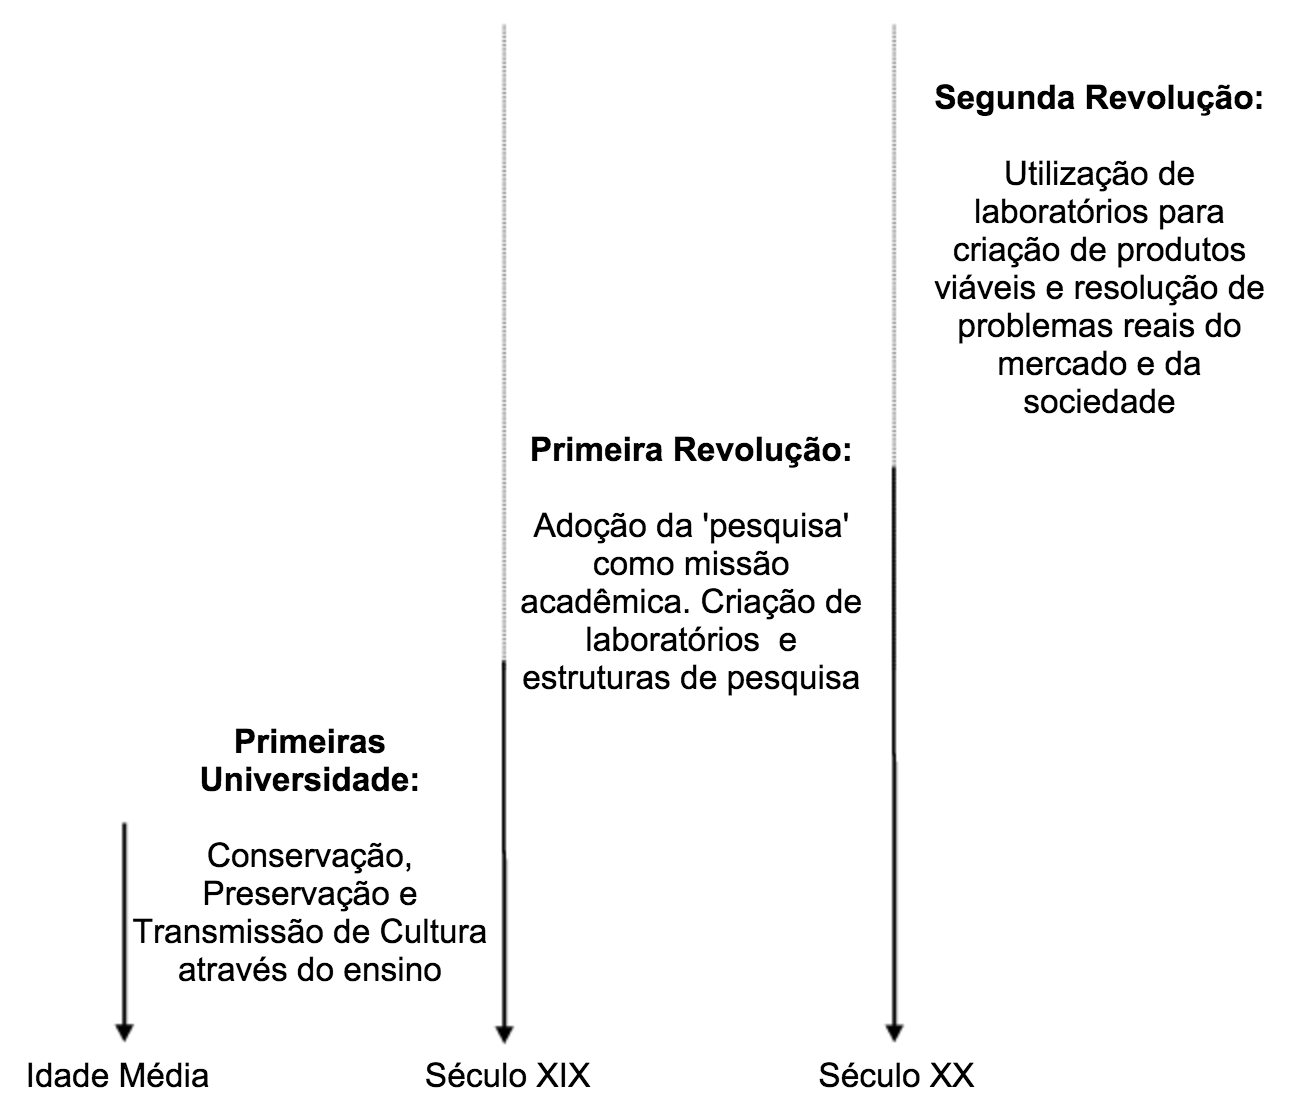
\includegraphics[scale=0.5]{img/academic_revolutions}}
\label{fig:academic_revolutions}
\caption* {Fonte: Elaborado pelo autor a partir de \citeonline{etzkowitz2001}}
\end{figure}

Com o advento da segunda revolução acadêmica, a universidade se capacitou a desenvolver soluções para problemas reais, seja através de pesquisas, projetos ou desenvolvimento de produtos. Um dos principais termos que foram cunhados posteriormente para caracterizar universidades que passaram a atuar diretamente na resolução de problemas para o governo e para a economia local e global foi o termo Universidade Empreendedora. O termo surgiu na academia em 1998, utilizado por Henry Etzkowitz e Burton Clark, e embora tenha sido publicado primeiramente por Etzkowitz, não há apropriação do termo pelo próprio autor.

Segundo \citeonline{etzkowitz1998}, a Universidade Empreendedora têm em sua base a \enquote{capitalização do conhecimento}, com a universidade apresentando uma conexão direta com usuários finais desse conhecimento, através de produtos ou serviços desenvolvidos por ela. Cria-se assim na universidade uma obrigação de identificar diretamente demandas do mercado para puxar inovações tecnológicas, ao passo que cada inovação deve ser devidamente apropriada pela universidade, através de seus direitos econômicos e intelectuais.

Já para \citeonline{burton}, a Universidade Empreendedora têm em sua base uma mudança organizacional da própria universidade, decorrente da globalização do conhecimento e da competitividade entre instituições de ensino. Com a evolução da tecnologia, em especial a difusão de informação através da internet, a transferência de conhecimento passou a acontecer com uma taxa cada vez maior deixando de acontecer localmente para tornar-se global. Criou-se um fácil acesso ao conteúdo e metodologia utilizados pelas universidades, além das pesquisas e resultados obtidos, fazendo com que a atuação da universidade na resolução de problemas do mercado se tornasse um diferencial competitivo de uma instituição em relação a outra.

O surgimento de Universidades Empreendedoras tem como consequência o aumento de interações entre Universidade e Empresa. As necessidades e expectativas em relação ao outro se transformaram de uma formação de profissionais e divulgação de pesquisas para uma série de parcerias em financiamento de projetos e laboratórios de pesquisa, com participação ativa de ambas as partes.

Não obstante, as Universidades Empreendedoras não só impulsionaram a frente de pesquisa como acabaram por modificar a estrutura curricular do ensino. Disciplinas de empreendedorismo e resolução de problemas foram adotadas pelas universidades que antes se apegavam ao modelo mais teórico. Segundo \citeonline{jeeModels}, o ensino de engenharia chegou a um estágio em que pode ser dividido em 3 principais modelos: Acadêmico, Market-Driven e Integrativo.

\begin{table}[H]
\begin{center}
\caption{Modelos de ensino de engenharia}
\label{tab:modelos_ensino_tab}
{\def\arraystretch{2}\tabcolsep=10pt
\begin{tabular}{>{\raggedright}p{0.2\linewidth}>{\raggedright\arraybackslash}p{0.2\linewidth}>{\raggedright\arraybackslash}p{0.2\linewidth}>{\raggedright\arraybackslash}p{0.2\linewidth}}
\hline
     & Modelo Acadêmico & Modelo \textit{Market-Driven} & Modelo Integrativo \\ \hline
     Percepção de Engenharia & Ciência Aplicada & Inovação Tecnológica & Serviço Público \\
     Papel Social & Consultor, Especialista & Empreendedor, Gestor & Cidadão, Agente de Mudanças \\
     Perspectiva Institucional & Universidade Científica & Universidade Empreendedora & Universidade Ecológica  \\
	 Exemplos de Disciplinas & Cálculo, Estatística & Empreendedorismo, Desenvolvimento de Produto & Sustentabilidade, Problemas da Sociedade \\ \hline
\end{tabular}%
}
\caption* {Fonte: Adaptado de \citeonline{jeeModels}}
\end{center}
\end{table}

O modelo acadêmico consiste no ensino de disciplinas básicas de caráter científico, responsável por formar especialistas nas respectivas áreas de conhecimento. O modelo \textit{market-driven}, conforme o nome já indica, é orientado pelas demandas tecnológicas do mercado. Logo abrange disciplinas de empreendedorismo e desenvolvimento de produtos, que somente com a formação de universidades empreendedoras foram incorporados à grade curricular de cursos de engenharia. Por fim existe o modelo integrativo, que corresponde a demandas da sociedade e do governo, que visa conscientizar e incentivar os alunos a resolverem problemas de cunho social. Esse é um modelo mais moderno, que enxerga no aluno um investimento feito pela sociedade que poderia trazer um retorno mais direto além do realizado através do mecanismo padrão de geração de valor dentro de uma empresa no mercado de trabalho. 

Dificilmente serão encontradas universidades que são adeptas de um modelo apenas, e sim um modelo híbrido das três partes. De toda forma, é importante ressaltar o papel de uma universidade ao estruturar sua forma de ensino, se estão de acordo com os objetivos e o papel social que ela quer exercer.

\subsection{Modelo Tripla Hélice}
\label{cha:univ_empreend}

Com o surgimento das Universidades Empreendedoras e o aumento das parcerias com Empresas, surge também a atuação do Governo como intermediador e facilitador dessas parcerias. A relação criada entre os 3 agentes com o objetivo de gerar desenvolvimento econômico local, direta ou indiretamente, é chamado de modelo Tripla Hélice. Nesse modelo, Governo, Empresa e Universidade atuam em um mesmo ecossistema na resolução de problemas reais através de soluções tecnológicas.

O peso e o papel de cada um dos três agentes da Tripla Hélice apresenta grandes variações conforme a localização do ecossistema ou a época da história em que se analisa a sua configuração. \cite{etzkowitz2000}

O primeiro modelo exemplificado pela Figura \ref{fig:triplehelix1} representa países  cujo regime possui influência absoluta do Estado, como na ex-União Soviética e países do Leste Europeu, em que o governo regula e direciona as relações entre as empresas e a academia de acordo com as suas necessidades. Esse modelo é amplamente visto como falho pois limita iniciativas de empresas e academia, desencorajando a inovação.

\begin{figure}[H]
\caption{Modelo de interação universidade-indústria-governo regulado pelo governo}
\centerline{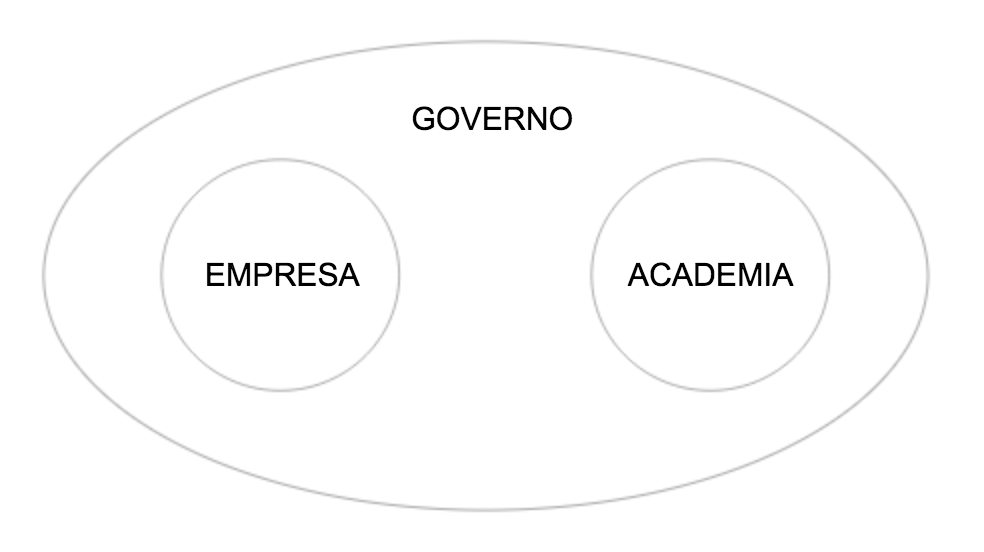
\includegraphics[scale=0.5]{img/triplehelix1}}
\label{fig:triplehelix1}
\caption* {Fonte: Adaptado de \citeonline{etzkowitz2000}}
\end{figure}

Um segundo modelo, apropriado da expressão \textit{laissez-faire}, símbolo do liberalismo econômico e da independência entre mercado e governo, consiste na minimização da interferência de atuação entre as esferas, principalmente em relação ao Governo, apresentando forte contraste em relação ao primeiro modelo. (Figura \ref{fig:triplehelix2}). Nesse modelo, cada ator atua de forma independente, apenas havendo transmissão de informação entre eles mas não uma colaboração ativa em prol da inovação.

\begin{figure}[H]
\caption{Modelo \textit{laissez faire}, de independência entre universidade, indústria e governo}
\centerline{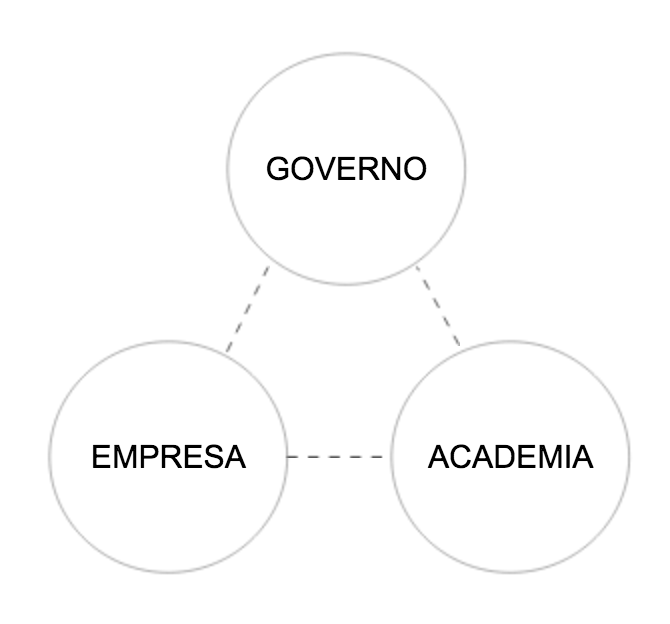
\includegraphics[scale=0.5]{img/triplehelix2}}
\label{fig:triplehelix2}
\caption* {Fonte: Adaptado de \citeonline{etzkowitz2000}}
\end{figure}

Já o terceiro modelo em questão representa uma infraestrutura de conhecimento compartilhada entre as esferas, com organizações híbridas surgindo nas interfaces entre as esferas, e consequentemente novas funções surgindo através da colaboração, cogestão e compartilhamento de recursos entre os atores. O autor considera esse modelo como o modelo tripla hélice propriamente dito, e o modelo referência adotado pela maioria das países e regiões que buscam uma parceria com muita informação nas interfaces entre as esferas. 


\begin{figure}[H]
\caption{Modelo Tripla Hélice Universidade-Empresa-Governo}
\centerline{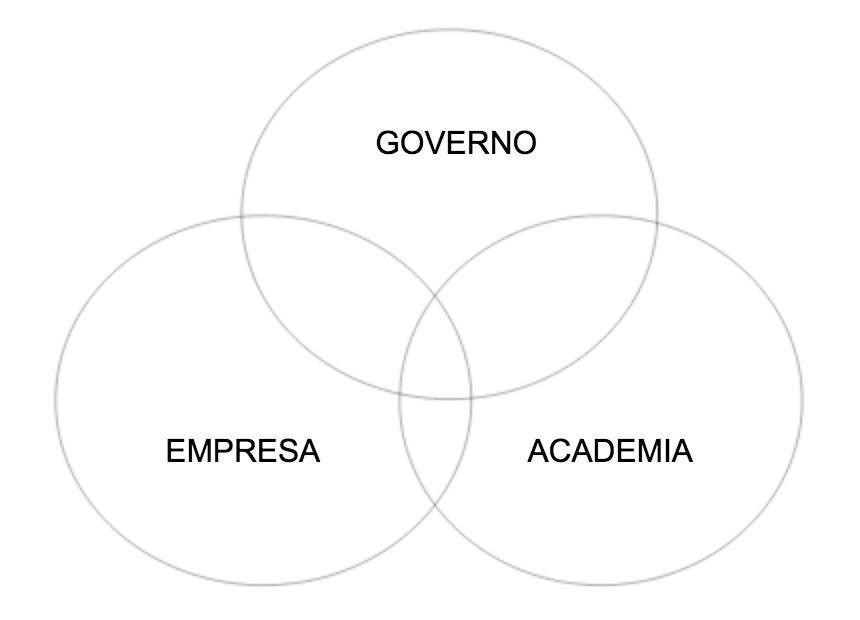
\includegraphics[scale=0.5]{img/triplehelix3}}
\label{fig:triplehelix3}
\caption* {Fonte: Adaptado de \citeonline{etzkowitz2000}}
\end{figure}

Dessa forma, é possível observar através do modelo de hélice tripla que grandes projetos de ensino, pesquisa e extensão devem ter participação ativa de Universidade, Empresa e Governo, pois todos estão interessados nos resultados diretos e indiretos dessa parceria.

\subsection{Contexto jurídico-legal para parceria universidade-empresa}
\label{cha:juridico_legal}

No modelo de tripla hélice o Governo assume uma posição de facilitador da interação entre empresa e academia sem tirar a autonomia de ambos os atores. Através de um contexto jurídico-legal fornecido pelo governo para intermediar as interações entre entidades, o governo viabiliza a captação de recursos para o desenvolvimento de novas pesquisas, e através da sua participação na criação de laboratórios e parques tecnológicos oferece uma infraestrutura para  auxiliar no processo de inovação.

No Brasil, de forma a incentivar a cultura, o esporte, o social e o desenvolvimento do país, foram criadas algumas leis de incentivo para empresas a investirem nessas frentes a troca de uma renúncia fiscal.  Normalmente, o governo abre mão de parte dos impostos da empresa pois os mesmos serão destinados a outros projetos de benefício da sociedade. Do lado da empresa é extremamente positivo, pois esse incentivo pode ser usado tanto para reforçar a imagem da empresa quanto para gerar um retorno financeiro, fatos que não ocorreriam caso o mesmo investimento fosse aplicado em forma de impostos.

Entre essas leis encontra-se a Lei 8.248/91, conhecida como lei da informática, que foi sancionada em Outubro de 1991 pelo então presidente Fernando Collor. Dentro desta Lei o principal benefício é a redução da alíquota do IPI de 15\% para 3\% até 2029. Em contrapartida, a empresa beneficiada por essa Lei se compromete a investir até 4\% do faturamento de determinado segmento em Pesquisa e Desenvolvimento. Também deve-se mencionar a lei 10.973/04, conhecida como Lei de Inovação Tecnológica, que estabelece incentivo financeiro para pesquisadores, de forma a \enquote{promover as atividades científicas e tecnológicas como estratégicas para o desenvolvimento econômico e social}.

\subsection{Desafios da gestão universidade-empresa}
\label{cha:univ_empreend}

Com a formação cada vez maior de universidades empreendedoras e o consequente aumento da participação ativa na inovação tecnológica e em resolução de problemas nacionais, foi necessário criar-se toda uma infraestrutura dedicada a facilitar as interações universidade-empresa. Em muitos casos a participação direta do governo é muito baixa e cabe à própria Universidade buscar e formar novas parcerias com empresas, gerando, além uma nova fonte de investimento, uma forte sinergia entre entidades para trabalhar em cima de problemas comuns.

\citeonline{plonsky} ressalta um grande marco ocorrido na época, que foi a mudança de ênfase da discussão sobre a cooperação entre academia e setor produtivo, com os debates evoluindo de questões como \enquote{será que universidade e empresa devem atuar em conjunto?} para questões relacionadas a como realizar a melhor gestão dessa parceria. De forma a elucidar essa questão ele define alguns principais desafios gerenciais entre universidade e empresa para manter a relação entre ambos \enquote{benéfica e transformadora}:

\begin{itemize}
\item Compartilhar uma visão multidimensional e integrada da cooperação universidade-empresa, centrada no desenvolvimento de competências humanas
\item Perceber com clareza as missões distintas, mas complementares, da empresa e da universidade no processo de inovação
\item Desenvolver respostas inovativas às diversas necessidades de cooperação empresa-universidade
\item Capacitar para a gestão eficaz da cooperação empresa-universidade
\end{itemize}

Primeiramente, ambos os lados devem entender que a parceria entre academia e empresa não se limita a projetos específicos e pontuais envolvendo ambas as partes, pois na realidade a parceria se extende a um dos principais objetivos da universidade, que é o de desenvolver alunos para atuar no mercado de trabalho. De forma geral, o setor produtivo deve estar sempre estar interessado na qualidade e na atualização do ensino das universidades pois consequentemente serão formadas pessoas mais capacitadas.

Em seguida, deve ficar evidente que empresa e universidade possuem papéis distintos no processo de inovação. A universidade assume na inovação o papel de organizar todo o conhecimento em relação a determinados assuntos. Já o desenvolvimento de tecnologia corresponde à aplicação do conhecimento organizado na produção de bens e serviços e, de forma geral, é de responsabilidade da empresa.

Embora existam diferentes necessidades de ambas as partes advindas da parceria universidade-empresa, deve-se compreender que por mais que a relação seja assimétrica, uma verdadeira cooperação não só deve ser benéfica como também deve gerar aprendizado para ambas as partes. Logo as respostas inovativas devem surgir mais rapidamente com ambos os lados sendo capacitados e beneficiados.

Por fim, todo caso de cooperação empresa-universidade deve estar sob gestão de um \textit{staff} pré-capacitado, pois uma série de conhecimentos acabam sendo necessários para tirar o máximo de proveito dessa parceria, como: desdobramento de missão e visão institucional; proteção de propriedade intelectual; equacionamento econômico-financeiro, gestão de projetos, entre outros.

\section{\textit{Benchmarking} de parcerias universidade-empresa:} % (fold)
\label{sec:cases}

De forma a ilustrar o funcionamento de parcerias entre Universidade e Empresa, foram selecionados alguns exemplos considerados bem-sucedidos. Os parques tecnológicos representam modelos bastante complexos pois envolvem um grande incentivo do governo para viabilizar a infraestutura, e uma participação extremamente ativa por parte das empresas que serão incubadas pelo parque. Por esse motivo foram selecionados dois dos principais parques tecnológicos nacionais para evidenciar todas as interações diretas e indiretas existentes para viabilizar a incubação de uma empresa.

Outro caso particular que foi selecionado para adicionar aos parques tecnológicos é a \textit{Deutsche Telekom} e os laboratórios estabelecidos em várias universidades para estabelecer parcerias de pesquisa na área de telecomunicação. Diferentemente dos parques tecnológicos que possuem uma grande infraestrutura e uma participação ativa do Governo muito grande, os \textit{T-Labs} são estruturas financiadas e construídas pela própria empresa com o propósito de inovar a frente de telecomunicações com várias universidades na Europa e Estados Unidos.

\subsection{TECNOPUC}

Os parques tecnológicos são um movimento de apoio à inovação e empreendedorismo que têm crescido muito nos últimos anos no Brasil. Eles se referem a aglomerações de empresas de base tecnológica, que podem ser pequenas ou não, articuladas a universidades e centros de P\&D, possibilitando sinergias decorrentes da proximidade entre os atores. \cite{parquestecnologicos} 

No Brasil há varios parques tecnológicos de destaque, como o Porto Digital em Recife, o Parque Tecnológico de São José dos Campos, o Parque Tecnológico da UFRJ e o Parque Científico e Tecnológico da PUC-RS (TECNOPUC). Dentre esse parques, a TECNOPUC se mostra um excelente caso de sucesso entre universidade e empresa, estimulando a pesquisa e a inovação por meio de uma ação simultânea entre academia, instituições privadas e governo, sob gestão da própria universidade.

O TECNOPUC possui um portfólio de empresas multissetorial, focado em quatro principais áreas definidas a partir da competência acadêmica da Universidade, envolvendo grupos de pesquisa científica e tecnológica, cursos de pós-graduação e à existência de demanda da sociedade. (Figura \ref{fig:tecnopuc})

\begin{figure}[H]
\caption{Áreas de atuação do Tecnopuc}
\centerline{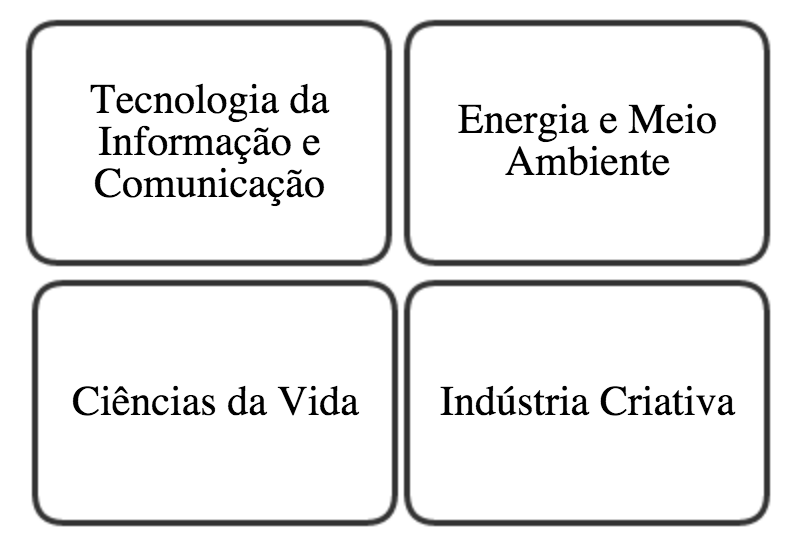
\includegraphics[scale=0.5]{img/tecnopuc}}
\label{fig:tecnopuc}
\caption* {Fonte: Adaptado do site do Tecnopuc}
\end{figure}

Atualmente, o TECNOPUC abriga 120 organizações, desde grandes companhias de tecnologia como Samsung, Microsoft, Motorola e Dell até instituições financeiras como o HSBC. 

O TECNOPUC é um dos pilares do INOVAPUCRS - Rede de Inovação e Empreendedorismo da PUC-RS. Segundo \citeonline{tecnopuc}, o sucesso da iniciativa de inovação e empreendedorismo na universidade se deve à combinação do TECNOPUC com diversas outras estruturas de apoio:

\begin{description}
\item[AGT] - A Agência de Gestão Tecnológica facilita e articula a comunicação entre empresa e pesquisadores, identificando possíveis parcerias, acelerando a burocracia inerente a essas parcerias e captando recursos para viabilizar os projetos
\item[ETT] - O Escritório de Transferência de Tecnologia é responsável pelo estabelecimento e proteção das diretrizes de propriedade intelectual das pesquisas geradas em parcerias com empresas.
\item[IDEIA] - O Instituto de Pesquisa e Desenvolvimento possui uma infraestutura laboratorial para incubar projetos de diversas unidades acadêmicas.
\item[RAIAR] - A Incubadora Raiar é responsável por abrigar empresas derivadas de pesquisas estabelecidas na universidade por alunos, professores ou funcionários ou novos empreendimentos de empresas já estabelecidas no TECNOPUC.
\item[LABELO] - Os Laboratórios Especializados em Eletroeletrônica trabalha na prestação de serviços tecnológicos, apoiando o fortalecimento e a qualificação dos produtos para atender a regulamentos e normas internacionais.
\item[CI] - O Centro de Inovação é uma parceria feita com a Microsoft de forma a acelerar o uso de novas tecnologias e fomentar a indústria de software.
\item[NE] - O núcleo empreendedor tem como objetivo estimular o empreendedorismo na Universidade através de palestras, eventos e projetos que visam as oportunidades de mercado e a inovação.
\end{description}

O TECNOPUC tem como missão criar uma comunidade de pesquisa e inovação transdisciplinar por meio da colaboração entre academia, empresas e governo visando aumentar a competitividade dos seus atores e melhorar a qualidade de vida de suas comunidades. Ele se baseia nos seguintes objetivos:

\begin{itemize}
\item Atrair empresas de pesquisa e desenvolvimento (P,D e I) para trabalhar em parceria com a Universidade
\item Promover a criação e o desenvolvimento de novas empresas de base tecnológica
\item Atrair projetos de pesquisa e desenvolvimento tecnológico em geral
\item Estimular a inovação e a interação empresas-Universidade
\item Gerar uma sinergia positiva entre o meio acadêmico e o empresarial
\item Atuar de forma coordenada com as esferas governamentais, particularmente no âmbito do Projeto Porto Alegre Tecnópole
\end{itemize}

\subsection{Porto Digital}

Assim como o TECNOPUC, o Porto Digital é um dos principais parques tecnológicos e ambientes de inovação do Brasil. Localizado no Recife, atua principalmente nos eixos de software e serviços de Tecnologia da Informação e Comunicação (TIC) e Economia Criativa (EC), com ênfase nos segmentos de games, multimídia, cine-vídeo-animação, música, fotografia e design.

O Porto Digital é referência nacional de adoção do modelo Tripla Hélice, pois é fruto de uma ação coordenada entre governo, academia e empresas. Essa iniciativa propiciou o ambiente necessário para fazer com que o Porto Digital se transformasse num dos principais ambientes de inovação do País. 

Atualmente, o Porto Digital abriga 250 empresas, organizações de fomento e órgãos de Governo e cerca de 7.100 trabalhadores, e foi considerado pela Associação Nacional de Promotoras de Empreendimentos Inovadores (Anprotec), em 2007 e 2011, o melhor parque tecnológico do Brasil. Em 2005 foi considerado o maior parque tecnológico do País pela A.T. Kearney.

O Plano de desenvolvimento de seu Arranjo Produtivo Local (APL) foi concebido a partir de 54 entrevistas com os seus principais \textit{stakeholders}:

\begin{itemize}
\item Núcleo de Gestão do Porto Digital (NGPD)
\item Conselho de Administração do NGPD
\item Instituições Locais (empresas embarcadas e não-embarcadas, órgão de representação de classes, governo estadual e municipal, instituições de ensino superior, entidades de fomento, imprensa e formadores de opinião)
\item Instituições não-locais (órgãos de representação de classe e de fomento)
\end{itemize}

A partir das informações obtidas nessas entrevistas, o plano estratégico do porto digital foi estruturado e pode ser representado pela figura \ref{fig:estrategiasPD}.

\begin{figure}[h]
\caption{Plano Estratégico do Porto Digital}
\centerline{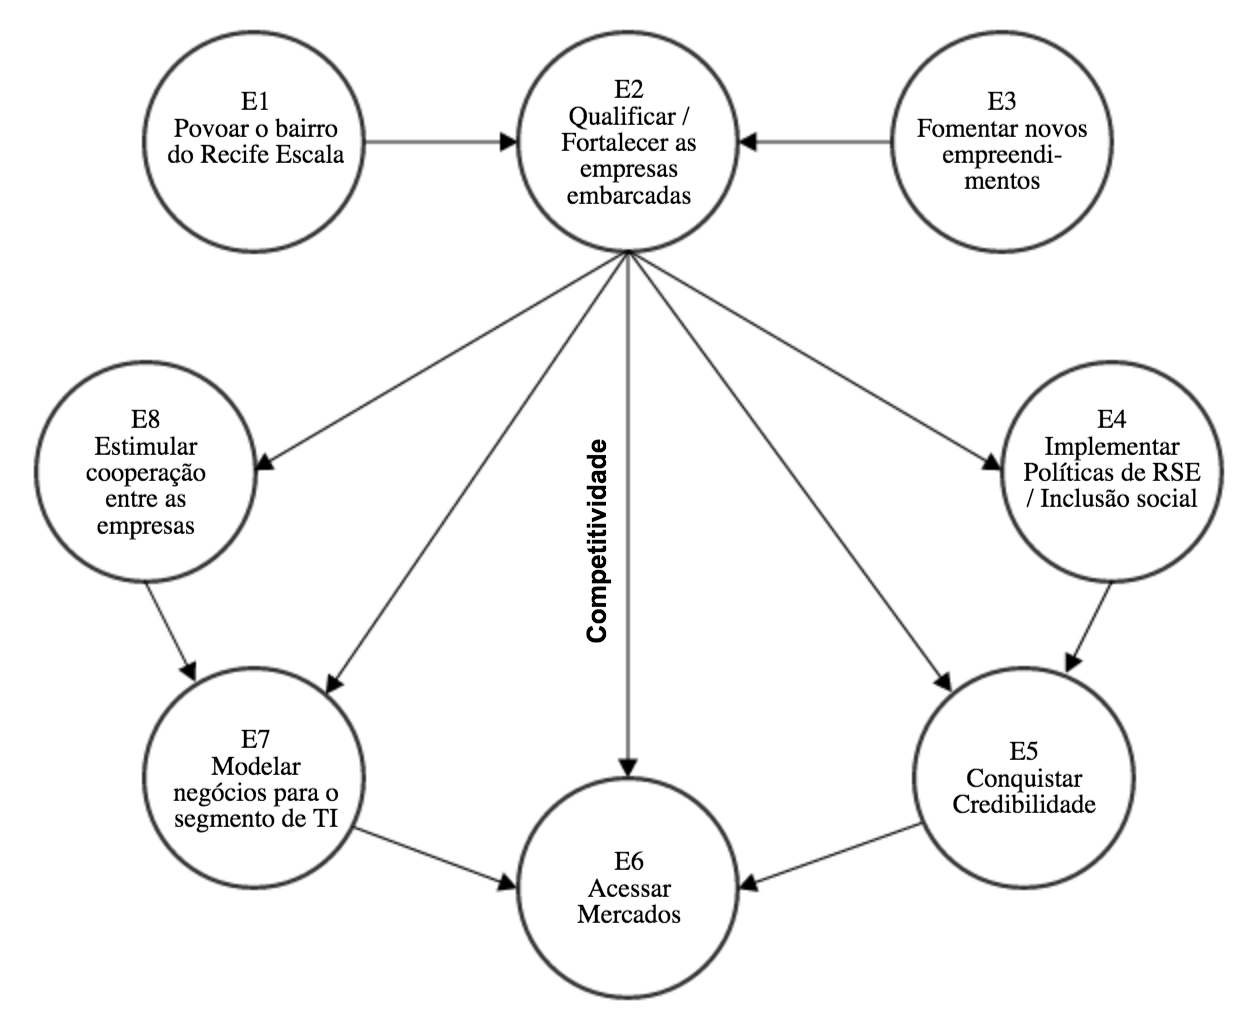
\includegraphics[scale=0.5]{img/estrategiasPD}}
\label{fig:estrategiasPD}
\caption* {Fonte: \citeonline{portodigital}}
\end{figure}

O eixo principal do plano consiste no fortalecimento das empresas (estratégia 2) para aumentar sua capacidade competitiva e viabilizar o acesso aos mercados nacionais e internacionais (estratégia 6). As demais estratégias atuam no sentido de aumentar a participação das empresas locais nos seus mercados. É importante ressaltar que não há hierarquia entre as estratégias fora do eixo central.

Basicamente, de forma a maximizar a qualificação das empresas embarcadas, é necessário que a economia local seja movimentada, gerando aumento de escala (estratégia 1) e que novos empreendimentos sejam fomentados para incentivar o APL e o setor de TIC. 

Já o acesso aos mercados depende muito da competitividade das empresas do Porto Digital. Para tal, é necessário que haja estímulo à cooperação entre as empresas do ambiente (estratégia 8), que possibilita a modelagem de novos negócios para o segmento, e a implementação de políticas de Responsabilidade Social Empresarial (RSE) e Inclusão Social (estratégia 4) auxiliam na conquista da credibilidade (estratégia 5).

O Plano Estratégico após concebido foi desdobrado em 8 projetos (Figura \ref{fig:projetosPD}), com tempo de execução de 36 meses e orçamento de R\$ 30 milhões, seguindo a metodologia do PMBOK. 

\begin{figure}[h]
\caption{Desdobramento de Projetos do Porto Digital}
\centerline{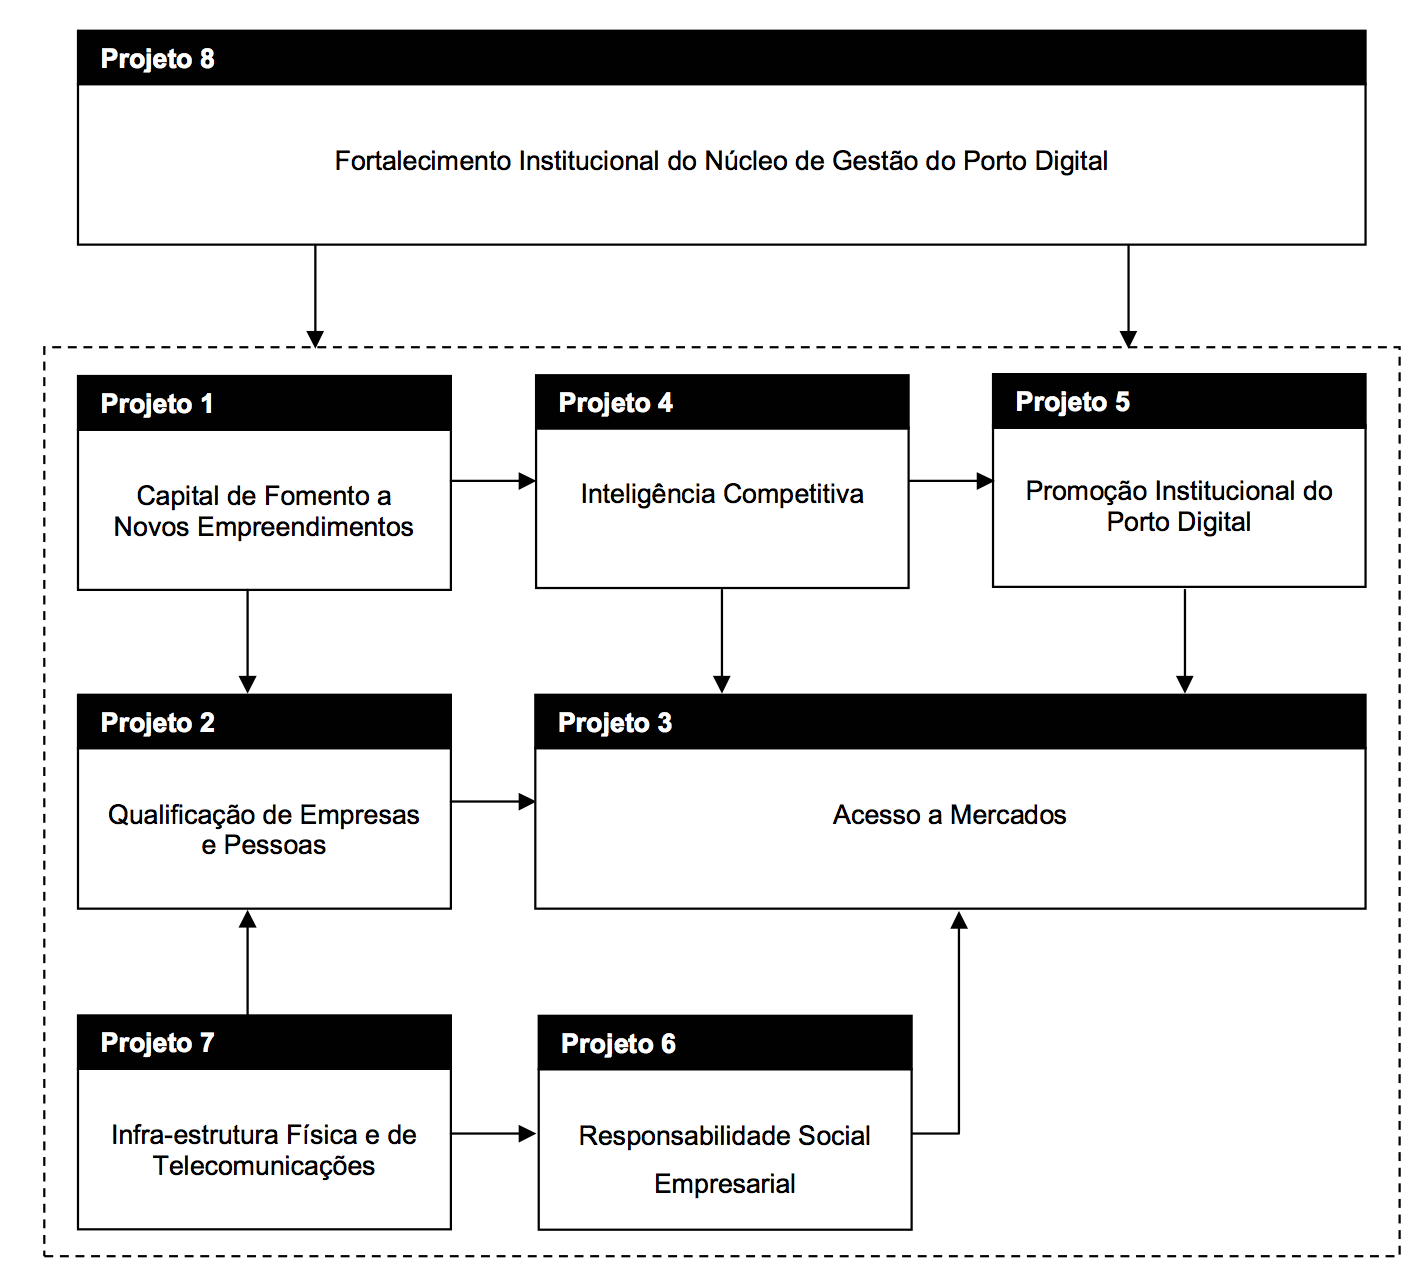
\includegraphics[scale=0.5]{img/projetosPD}}
\label{fig:projetosPD}
\caption* {Fonte: \citeonline{portodigital}}
\end{figure}

Para concretizar todo esse planejamento, o Porto Digital formalizou parcerias tanto na frente acadêmica (UFPE, UPE, Senac) quanto do lado do Governo (Prefeitura de Recife e Olinda, Secretarias de Desenvolvimento Social e Cidadania e Educação). Cerca de 35\% dos colaboradores com curso superior são alunos da UFPE.

\subsection{\textit{Deutsche Telekom - T-labs}}

A \textit{Deutsche Telekom} (DT) é uma empresa de telecomuniçação Alemã e também a maior do setor em toda a União Européia. A companhia possui um grande expertise na área de tecnologia da comunicação e tecnologia da informação, possuindo duas grandes subsidiárias: a operadora T-mobile e a consultoria de TI T-Systems, ambas com atuação global.

Por atuar em um segmento tão competitivo e totalmente dependente de inovações tecnológicas para gerar vantagem competitiva diante das outras empresas, a DT sempre apresentou muitas iniciativas e um forte investimento na área de P\&D. Através de uma dessas iniciativas surgiu a proposta dos Laboratórios \textit{Deutsche Telekom} (T-labs).

Os T-labs foram criados com o objetivo de pesquisar e desenvolver Tecnologia da Informação e Tecnologia da Comunicação de forma a permitir que novos negócios surjam e que operações já existentes sejam expandidas e acelerar o processo de inovação através da colaboração indústria e academia. \cite{dtlabs}

Para validar a real necessidade da DT em criar os laboratórios, foram levantadas as motivações apresentadas na tabela \ref{tab:motivacoes_dt}

\begin{table}[h]
\begin{center}
\caption{Fontes de Motivação para fundação dos T - Labs}
\label{tab:motivacoes_dt}
\begin{tabular}{>{\raggedright}p{0.25\linewidth}>{\raggedright\arraybackslash}p{0.55\linewidth}}
	\hline
    Importância & Indústria \\ 
    \hline \\
    \multirow{2}{*}{Razão Principal} 
    & Acesso à Inovação \\
    & Obter na fonte últimos avanços tecnológicos \\ \\
	\multirow{2}{*}{Alta importância}
	& Constante atualização do \textit{know-how} \\
	& Canal de Recrutamento \\ \\
	\multirow{2}{*}{Média importância}
	& Diminuição de risco com pesquisas \\
	& Estabelecer projetos de longo prazo \\ \\
	\multirow{2}{*}{Baixa importância}
	& Diminuição de custos \\
	& Uso de laboratório \\ \\
\end{tabular}%
\caption* {Fonte: \citeonline{dtlabs}}
\end{center}
\end{table}

De forma geral, a DT buscava nos laboratórios uma porta de entrada para descobertas e inovações tecnológicas, além de possíveis novos funcionários e pesquisas de longo prazo.

Dadas as necessidades listadas, a DT sabia que o próximo passo para viabilizar o laboratório seria ultrapassar algumas barreiras existentes em parcerias universidade-empresa: barreiras culturais, institucionais e operacionais. \cite{barriers}

Em relação às barreiras culturais, foram definidos três principais pontos:
\begin{itemize}
\item Apenas são empregados pós doutorados com interesse em pesquisa orientada pela aplicação dos resultados da pesquisa
\item Políticas de publicação e de direito à propriedade intelectual foram bem definidas, com prazos e condições bem descritos
\item Compartilhamento de espaço físico e políticas internas tanto para o \textit{staff} acadêmico quanto da indústria.
\end{itemize}

Em relação às barreiras institucionais:
\begin{itemize}
\item Divisão de objetivos bem definida, com o \textit{staff} da academia voltado para a pesquisa estratégica, e o \textit{staff} da indústria voltado para atividades orientadas pelo desenvolvimento e inovação.
\item Resultados esperados pré definidos através de KPIs, de tal forma que cada área já sabe o que é esperado de si.
\item Separação e autonomia da gestão do laboratório por parte da empresa, de tal forma que mudanças corporativas na DT pouco interfiram no trabalho do laboratório.
\end{itemize}

Em relação às barreiras operacionais:
\begin{itemize}
\item Processos bem definidos 
\item Alinhamento entre áreas feito através da revisão trimestral de projetos e apresentações de progresso
\item Redução do princípio Não-Inventado-Aqui (NIA), no qual as corporações se recusam a usar soluções de terceiros para usar soluções desenvolvidas internamente.
\end{itemize}
